\documentclass[12pt]{article}
\usepackage[margin=1in]{geometry}
\usepackage[all]{xy}
\usepackage{color}
\usepackage{enumerate}
\usepackage{amsmath,amsthm,amssymb,color,latexsym}
\usepackage{geometry}        
\usepackage{graphicx}
\usepackage{caption}
\usepackage{float}
\usepackage{stfloats}
\newtheorem{parter}{Part}
\newtheorem*{efficiency}{Efficiency}
\newtheorem*{example}{Example}
\newtheorem{step}{Step}
\newenvironment{solution}


\begin{document}
\noindent ECS 174 Spring 2020 \ (05/11)\hfill Problem Set \#2\\
Bingwei Wang \ 914683636\\
Nan Chen \ 915218152

\hrulefill

\begin{parter}
\end{parter}
    
\begin{solution}
    \begin{itemize}
        \item [(1)]We believe that the grouping algorithm graph-cuts, would be the most appropriate grouping algorithm to recover the model parameter hypotheses from the continuous vote space. The reason is that it links every pair of pixels and assigns an affinity weight for each edge. 
        \\
        Also, graph-cuts connect shapes with edges that have high affinity while mean shift and k-means does not, which suits those lines and circles defined by a set of boundary points in Hough Transform.
        \item [(2)]From using K-means clustering with two groups, we will have two center points which divides all the feature inputs into two clusters. Each center point will get half of the feature points and the center point will be positioned by calculating the least squared Euclidean distance. After that it will updates the new center of each cluster. The process will keep repeated until half of the data points are in one group and the other half is in the other group.
        \item [(3)]TO BE CONTINUE. {$\square$}
    \end{itemize}
\end{solution}

\begin{parter}
\end{parter}
    
\begin{solution}
    \begin{itemize}
        \item [(a)]The code is written in file \textbf{get\_correspondences.m}. The function has two inputs of two images and the number of points the user wants to pick. The outputs are two 2 x N point matrices of selected points.
        \item [(b)]The code is written in file \textbf{computeH.m}.
        \item [(c)]The code is written in file \textbf{warpImage.m}.
        \item [(d)]Images:
        \begin{figure}[H]
            \centering
            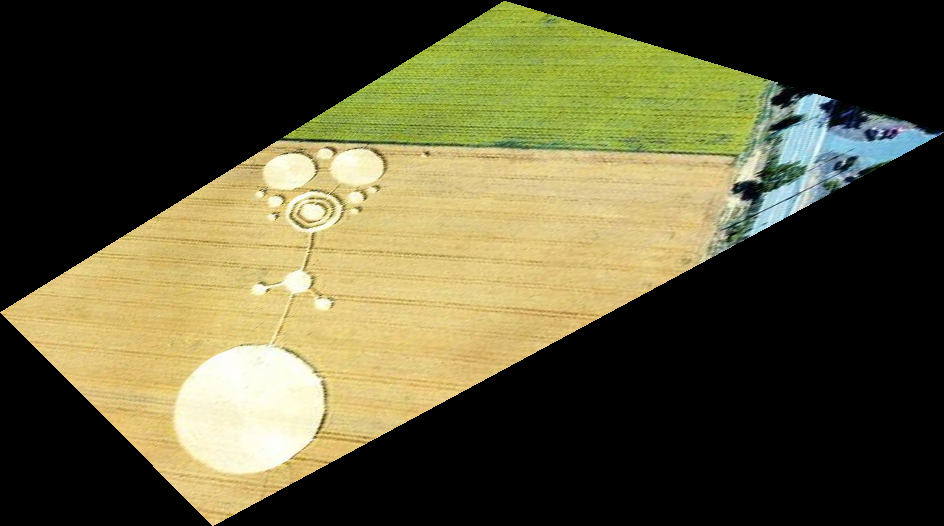
\includegraphics[width=16cm, height=10cm]{../cropwarp.png}
            \caption{crop\_warp}
        \end{figure}
        \begin{figure}[H]
            \centering
            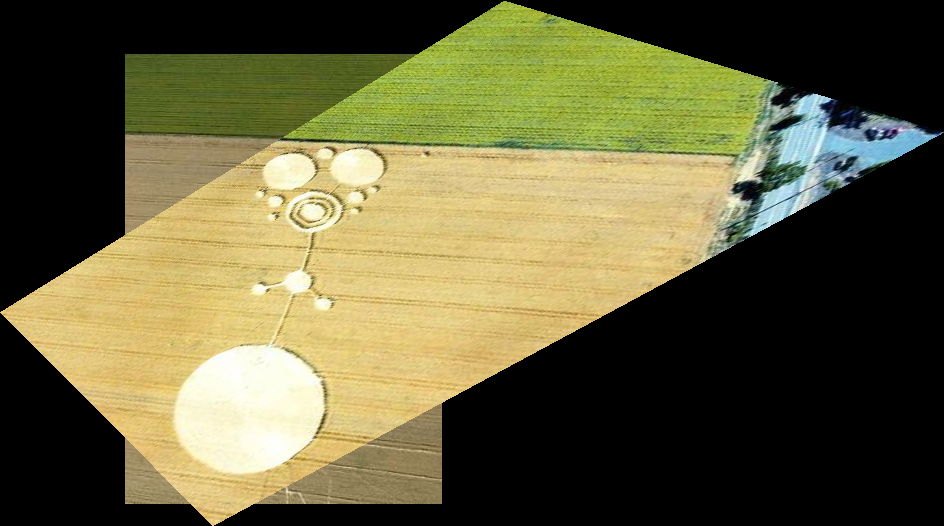
\includegraphics[width=16cm, height=10cm]{../cropmos.png}
            \caption{crop\_merge}
        \end{figure}
        \begin{figure}[H]
            \centering
            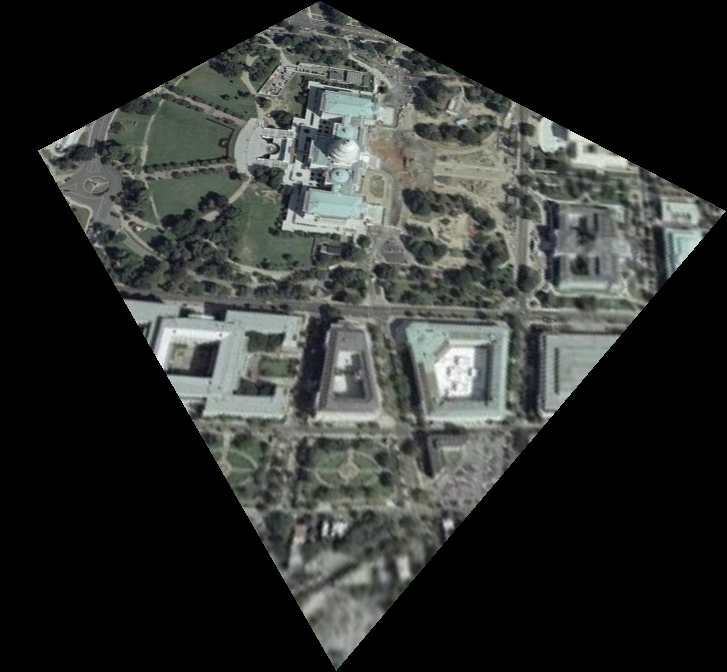
\includegraphics[width=10cm, height=12cm]{../wdcwarp.png}
            \caption{wdc\_warp}
        \end{figure}
        \begin{figure}[H]
            \centering
            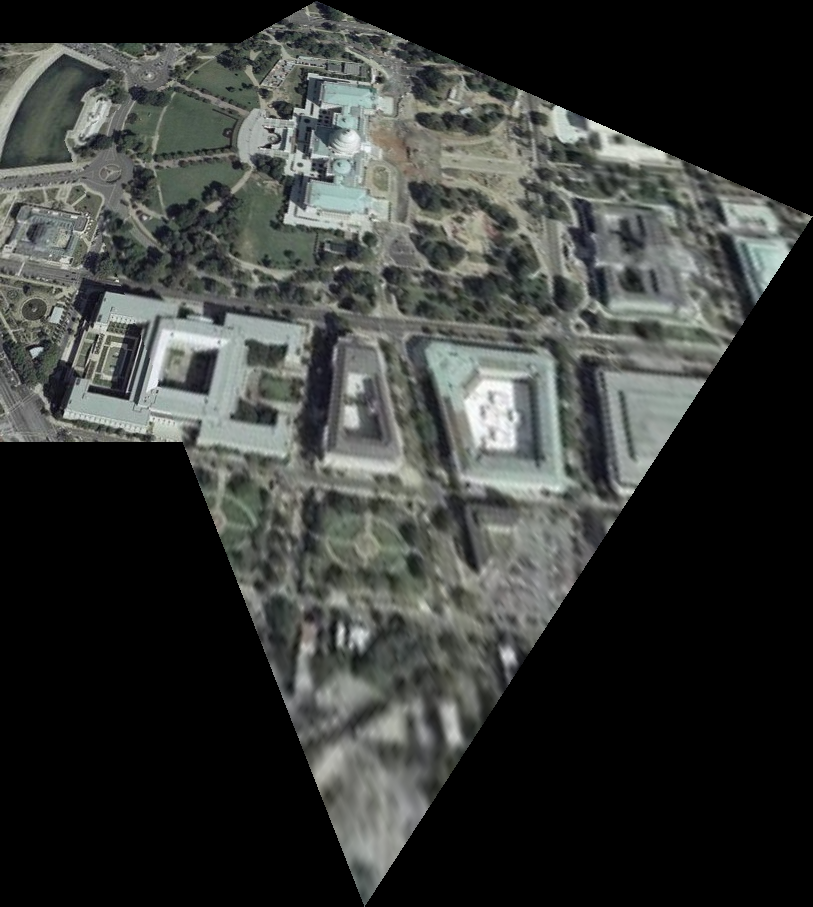
\includegraphics[width=10cm, height=12cm]{../wdcmos.png}
            \caption{wdc\_merge}
        \end{figure}
        The data points1 and points2 are saved in the file \textbf{points.m}.
        \item [(e)] Images:
        \begin{figure}[htbp]
            \centering
            \begin{minipage}[t]{0.48\textwidth}
            \centering
            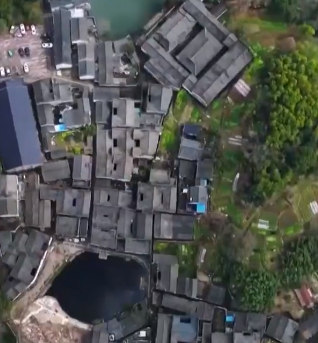
\includegraphics[width=5cm, height=6cm]{../town1.png}
            \caption{town\_source\_1}
            \end{minipage}
            \begin{minipage}[t]{0.48\textwidth}
            \centering
            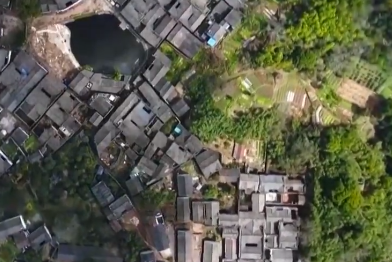
\includegraphics[width=7cm, height=5cm]{../town2.png}
            \caption{town\_source\_2}
            \end{minipage}
        \end{figure}
        \begin{figure}[H]
            \centering
            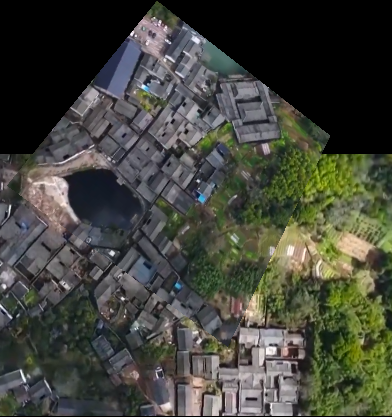
\includegraphics[width=11cm, height=12cm]{../townmos.png}
            \caption{town\_mosic}
        \end{figure}
        Source: https://www.bilibili.com/bangumi/play/ep264278.
        \item [(f)] Images:
        \begin{figure}[H]
            \centering
            
\includegraphics[width=15cm, height=5cm]{../plate.png}
            \caption{plate}
        \end{figure}
        \begin{figure}[H]
            \centering
            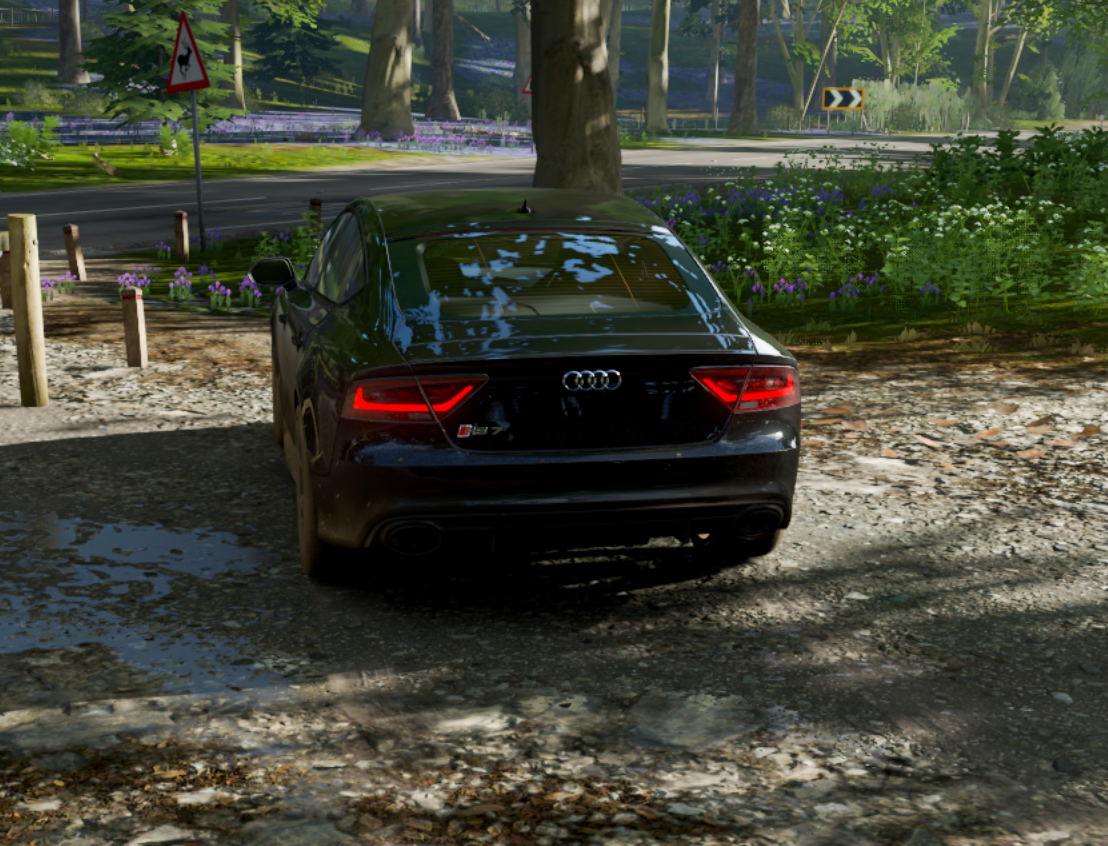
\includegraphics[width=15cm, height=12cm]{../car.png}
            \caption{car}
        \end{figure}
        \begin{figure}[H]
            \centering
            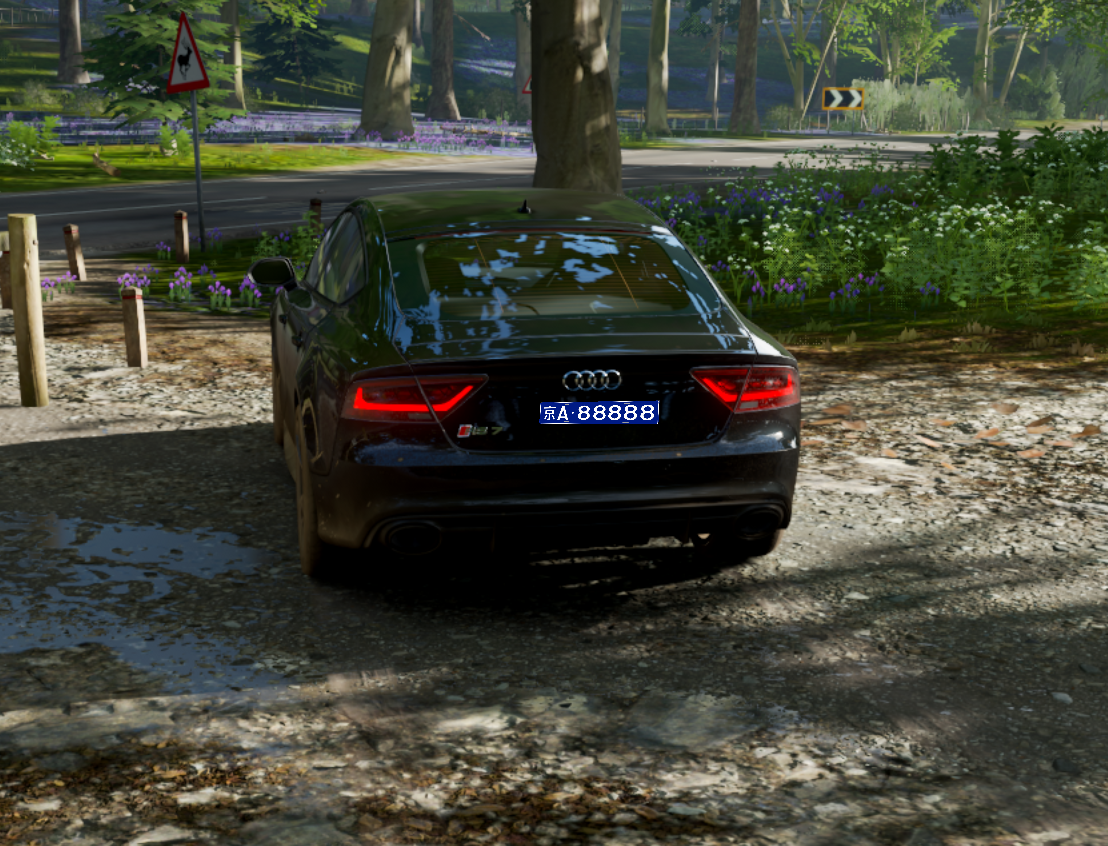
\includegraphics[width=15cm, height=12cm]{../carmos.png}
            \caption{car\_mosic}
        \end{figure}
        Source: ScreenShots from Game Forza Horizon4.\\
        Take the license plate picture, and mosic it on the car.
        {$\square$}
    \end{itemize}
\end{solution}

\begin{parter}
\end{parter}
    
\begin{solution}
    \begin{itemize}
        \item [(a)] Images:
        \begin{figure}[htbp]
            \centering
            \begin{minipage}[t]{0.48\textwidth}
            \centering
            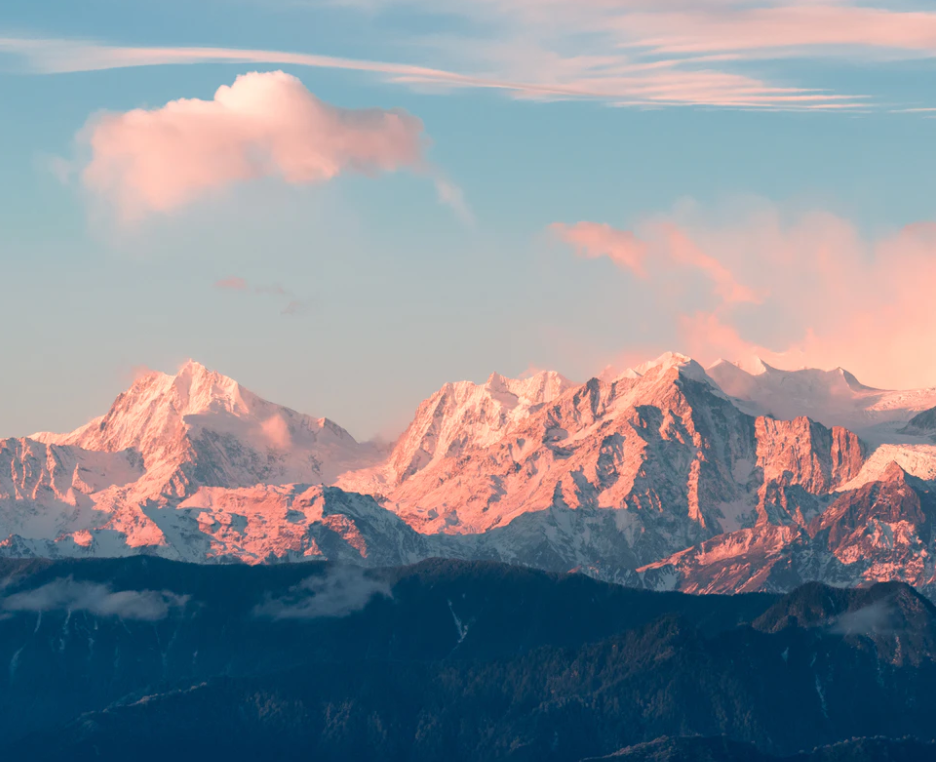
\includegraphics[width=6cm, height=7cm]{../mountain1.png}
            \caption{mountain\_source\_1}
            \end{minipage}
            \begin{minipage}[t]{0.48\textwidth}
            \centering
            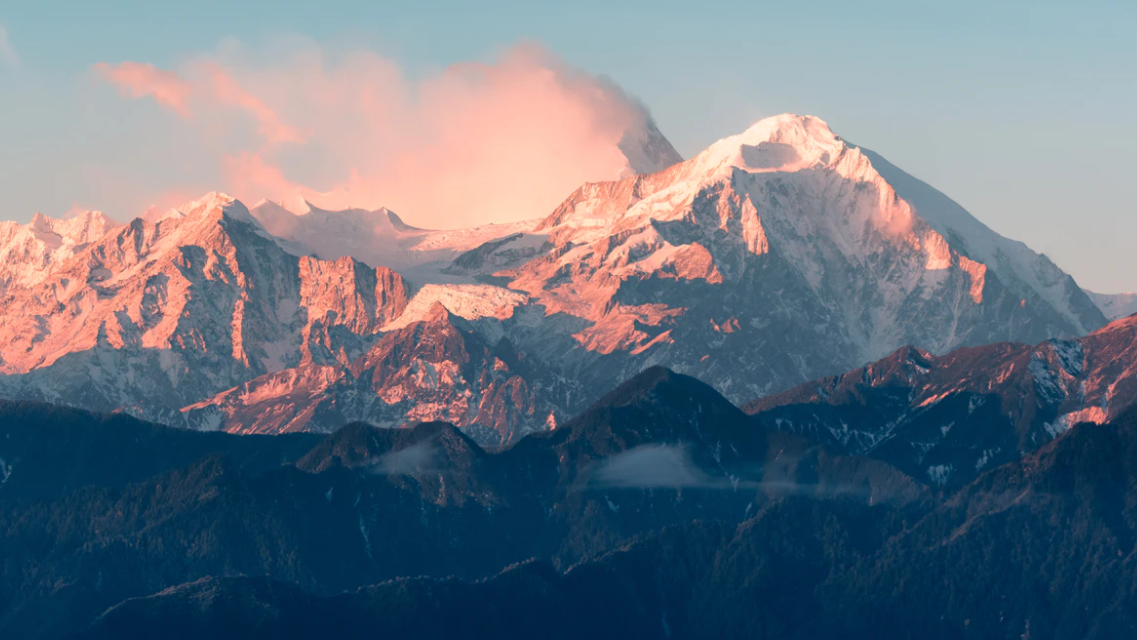
\includegraphics[width=7cm, height=5cm]{../mountain2.png}
            \caption{mountain\_source\_2}
            \end{minipage}
        \end{figure}
        \begin{figure}[htbp]
            \centering
            \begin{minipage}[t]{0.48\textwidth}
            \centering
            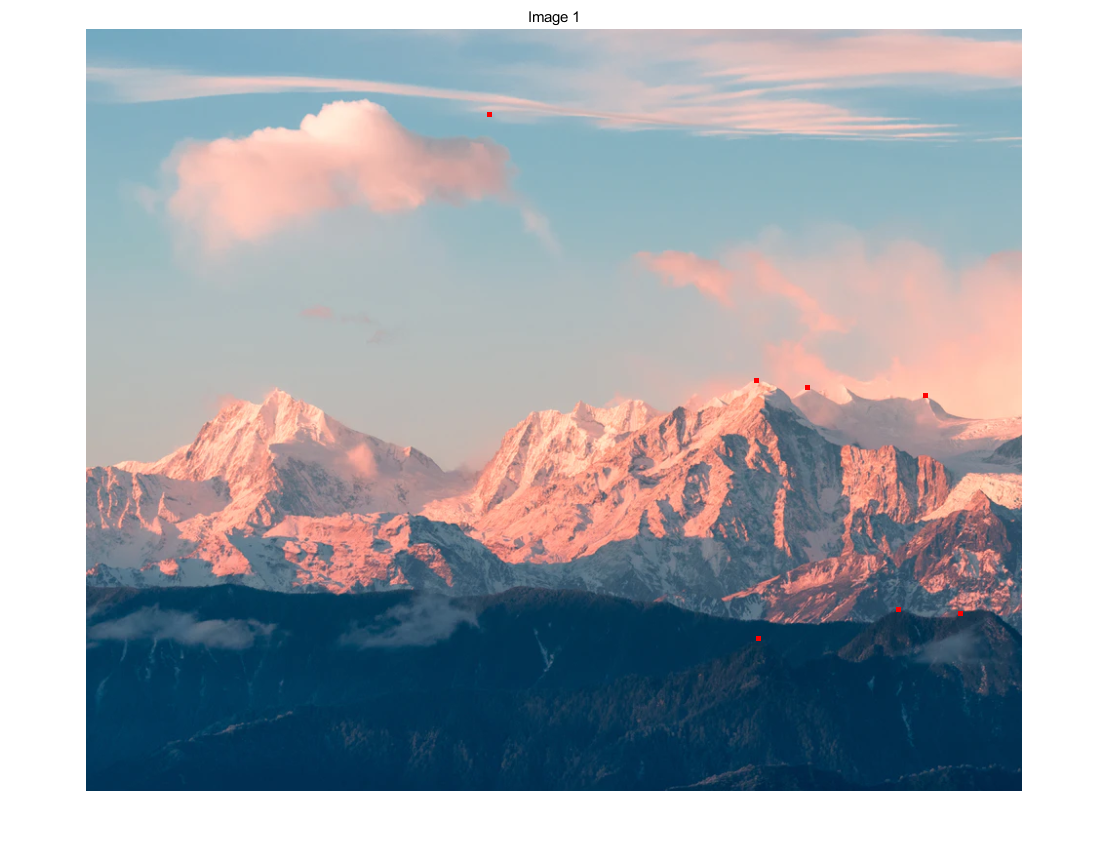
\includegraphics[width=6cm, height=7cm]{../mountain1_select.png}
            \caption{mountain\_select\_1}
            \end{minipage}
            \begin{minipage}[t]{0.48\textwidth}
            \centering
            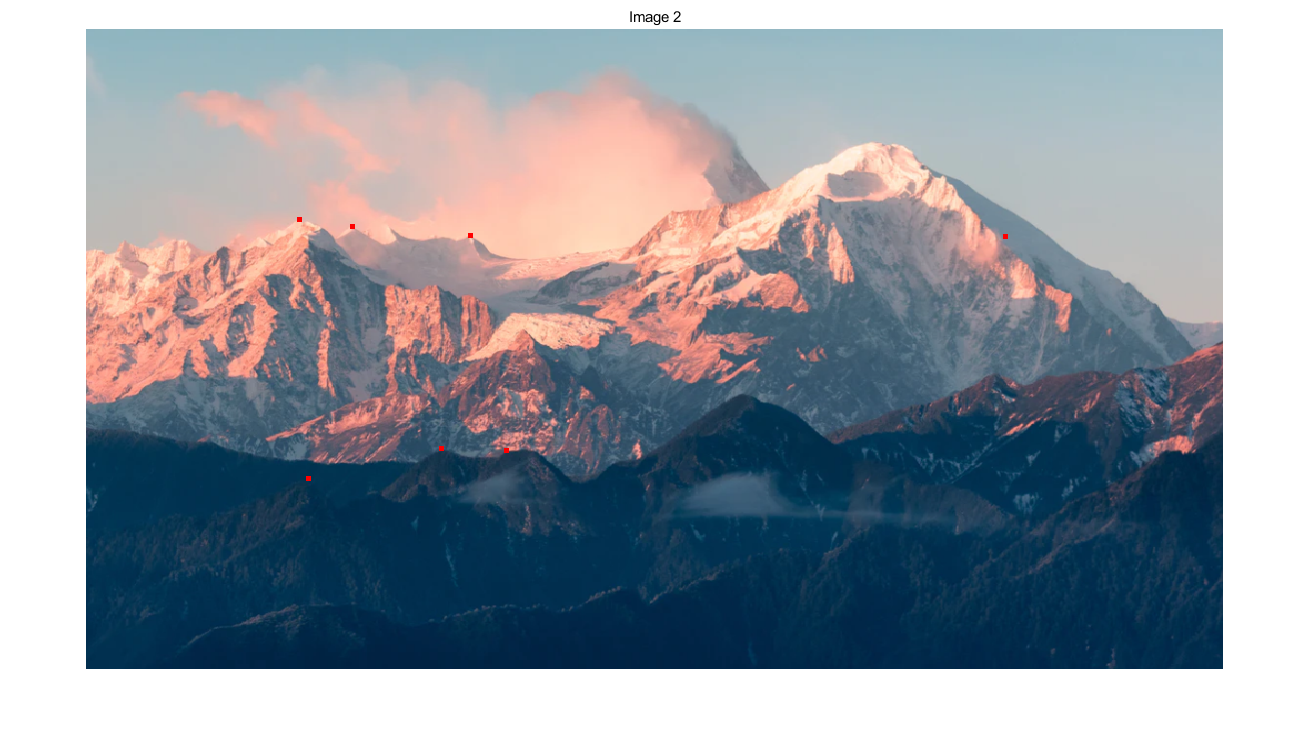
\includegraphics[width=7cm, height=5cm]{../mountain2_select.png}
            \caption{mountain\_select\_2}
            \end{minipage}
        \end{figure}
        \begin{figure}[H]
            \centering
            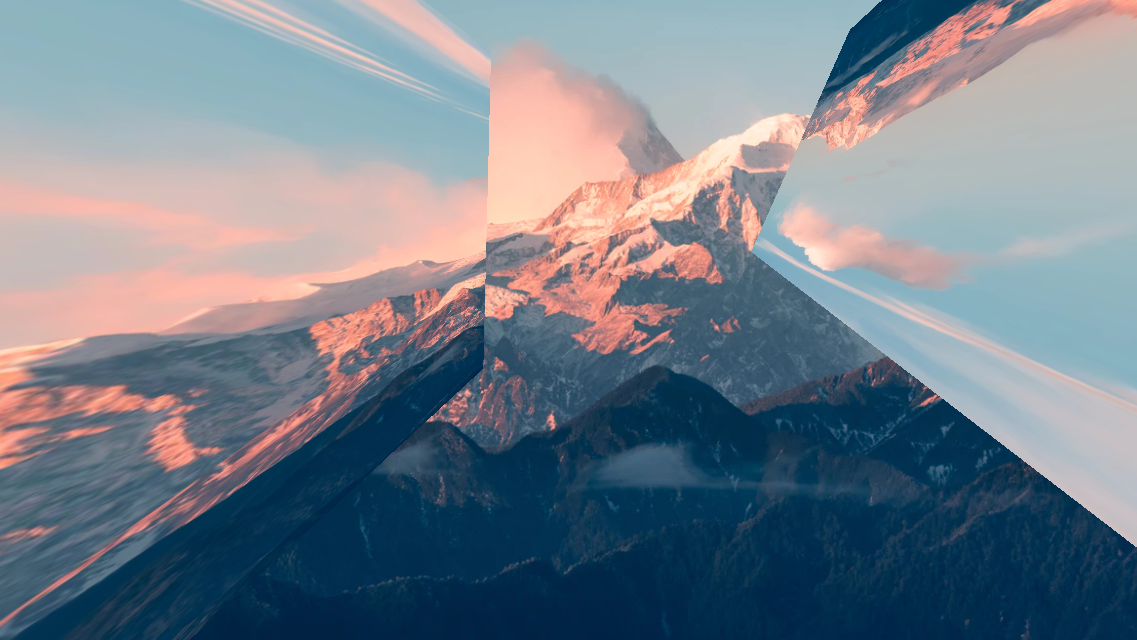
\includegraphics[width=15cm, height=12cm]{../mountainmos_O.png}
            \caption{mountain\_mosic\_original}
        \end{figure}
        \begin{figure}[H]
            \centering
            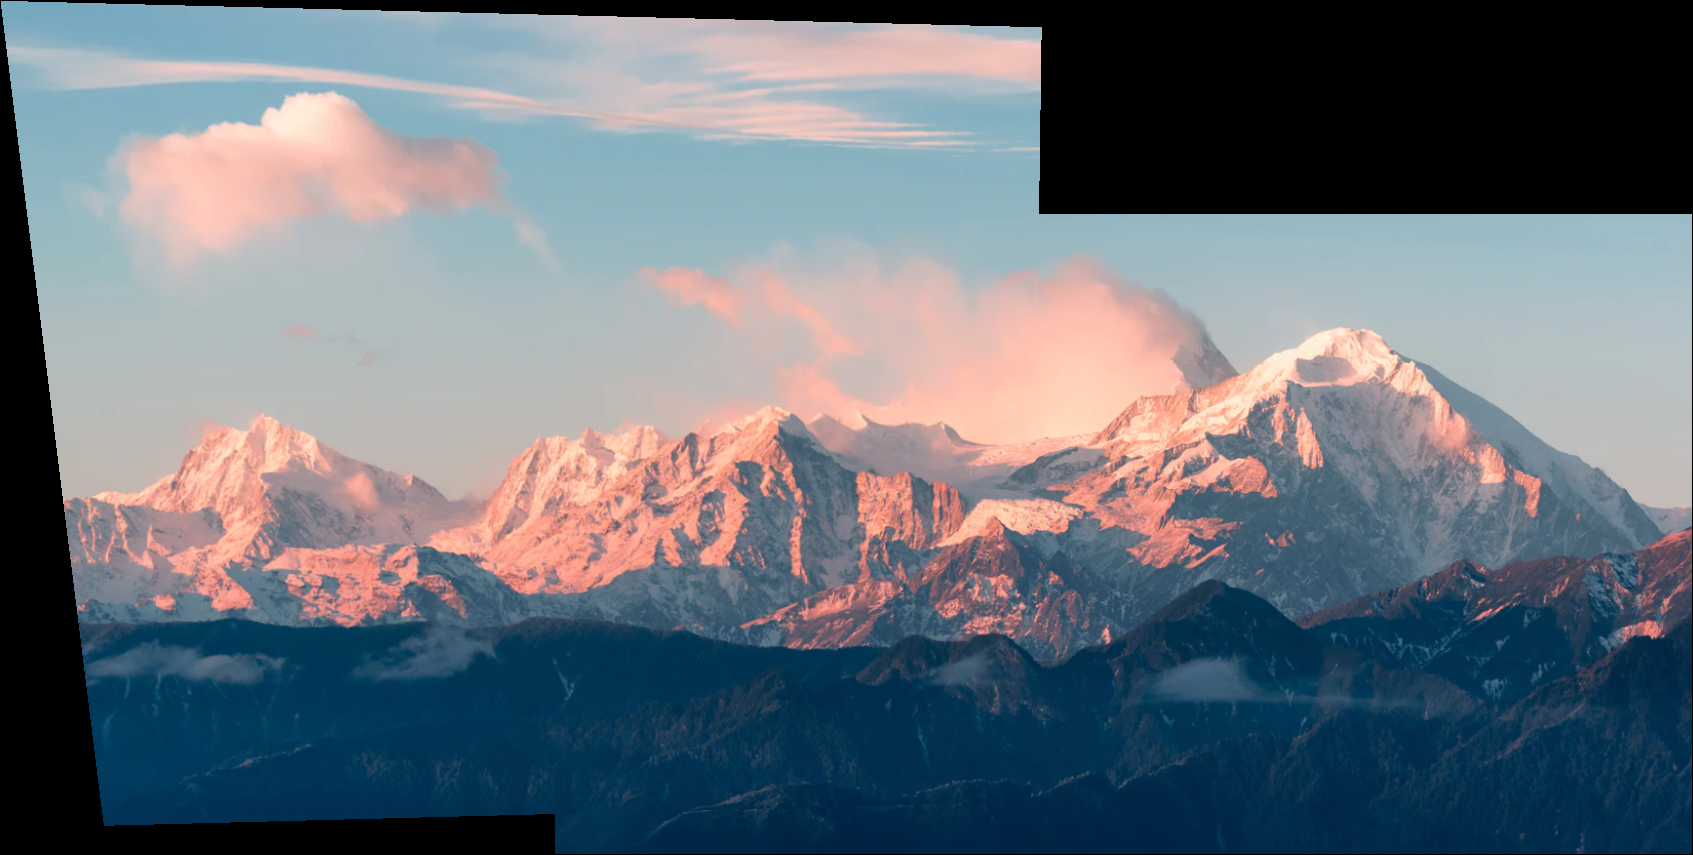
\includegraphics[width=15cm, height=12cm]{../mountainmos_R.png}
            \caption{mountain\_mosic\_RANSAC}
        \end{figure}
        Source: https://unsplash.com/photos/Y8lCoTRgHPE.\\
        TO Write Something.
        \item [(b)] Images:
        \begin{figure}[H]
            \centering
            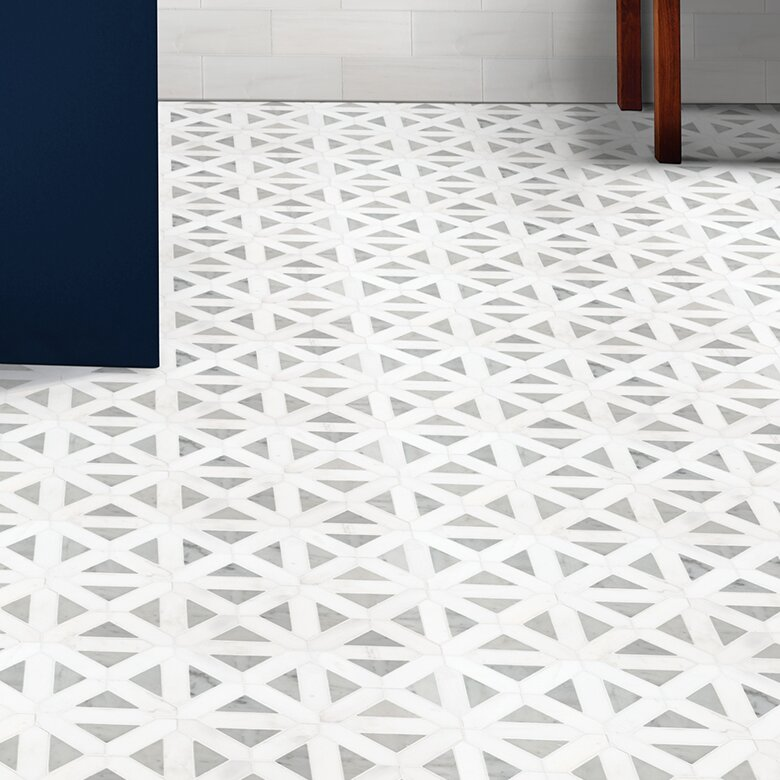
\includegraphics[width=15cm, height=12cm]{../tiles.jpg}
            \caption{tiles\_source}
        \end{figure}
        \begin{figure}[H]
            \centering
            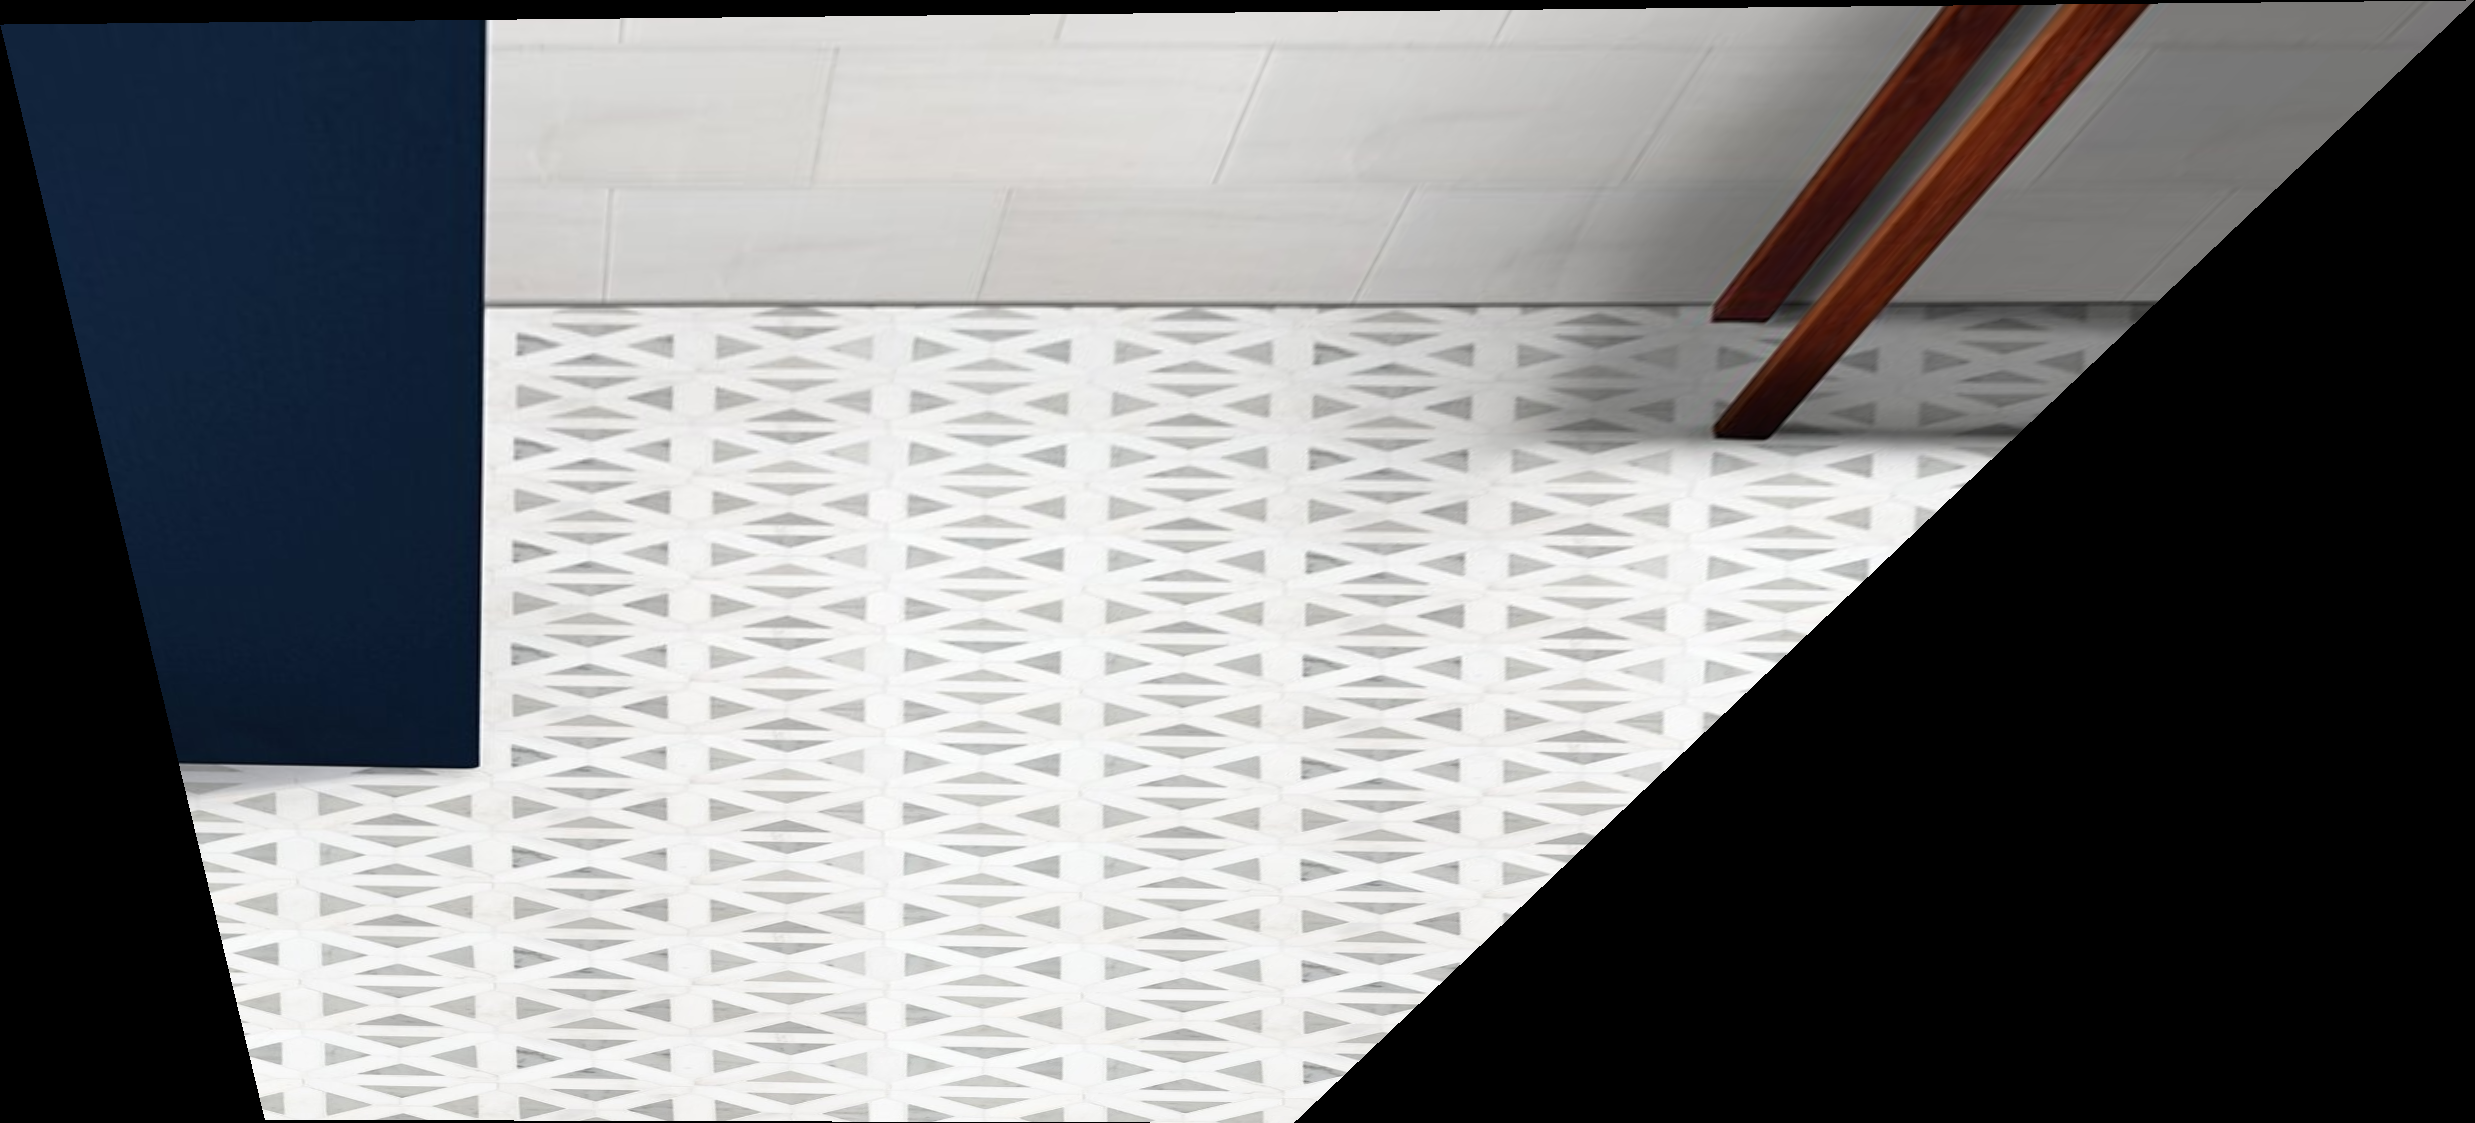
\includegraphics[width=15cm, height=12cm]{../tilesmos.png}
            \caption{tiles\_fronto}
        \end{figure}
        Source: https://www.wayfair.com/home-improvement/pdp/msi-bianco-dolomite-marble-mosaic-tile-mvp4112.html?piid=49665325.\\
        To Write Something.
        {$\square$}
    \end{itemize}
\end{solution}

\end{document}